\section{Experimentación}%
\label{sec:experimentacion}

% TL;DR; Intro experimentación.
En esta sección se incluye la experimentación llevada a cabo sobre nuestro
modelo de clasificador.

\subsection{Metodología}%
\label{sub:metodologia}
\subsubsection{Dependencia de factores}

Cuando consideramos una métrica de precisión como función objetivo de todos estos parámetros
no resulta manejable optimizar en un único paso de manera multivariada (son muchos)
ni tampoco analizar parámetro a parámetro dado que cada uno afecta como variable de manera
interpendiente a la función objetivo no pudiendo aislar un \textit{orden topológico}
de parámetros para optimizar de manera independiente.
En respuesta a esto se plantea un esquema de experimentación basado en aproximar
un orden de optimización de parámetros que sea relativamente parecido a un orden
topológico fijando algunos de ellos en valores intuitivos para eliminar dependencias
y poder seguir con las optimizaciones de a pares o por separado según sea conveniente
de manera de respetar lo máximo posible las dependencias.
Aunque solamente realizamos una iteración como prueba de concepto, este esquema
permite poder ir actualizando los valores que se fijan de manera iterativa incremental
mejorando paso a paso la función objetivo. El esquema en cuestión es:
\begin{itemize}
    \item buscar tolerancia de convergencia para método de la potencia (desempata candidatos con PCA con algunos parámetros fijos)
    \item buscar el k óptimo para kNN sin PCA en función de alguna vectorización fija
    \item buscar k y alfa óptimos para kNN con  PCA guiando el rango de k según el paso anterior nuevamente con vectorización fija
    \item buscar parámetros de vectorización óptimos para kNN según los parámetros anteriores
\end{itemize}


\subsection{Convergencia de método de la potencia}%
\label{sub:pm}
Como en cada k-ésima iteración del método de la potencia estamos consiguiendo un $v^{(k)}$ autovector tentativo asociado a un $\hat{\lambda}^{(k)}$ autovalor también tentativo podemos analizar su evolución para determinar si están convergiendo y cortar la iteración cuando ya lo consideremos suficiente. Dado un $\epsilon \in \mathds{R}$ tal que $\epsilon > 0$, la matriz cuadrada $A\in \mathds{R}^{n\times n}$ sobre la cual buscamos su autovalores, y los autovalores y autovectores tentativos de la k-ésima iteración $\hat{\lambda}^{(k)} \in \mathds{R}$ y $v^{(k)} \in \mathds{R}^{n}$ planteamos los siguientes criterios de corte:

\begin{itemize}
    \item Criterio de \textit{vector residual}: cortar si $|| A v^{(k)} - v^{(k)}\hat{\lambda}^{(k)} || < \epsilon$
    \item Criterio de diferencia de autovectores: cortar si $|| v^{(k)} - v^{(k-1)} || < \epsilon$
    \item Criterio de diferencia de autovalores: cortar si $|| \hat{\lambda}^{(k)} - \hat{\lambda}^{(k-1)} || < \epsilon$
\end{itemize}

Como bajo ciertas condiciones (como $|\lambda_1| \approx |\lambda_i|$ para $\lambda_1$ autovalor dominante y $\lambda_i$ otro autovalor de la matriz $A$) el método de la potencia puede no converger, al margen de los criterios se corta la iteración tras una cantidad fija y lo suficientemente grande (de modo que si converge no interrumpa a los criterios anteriores) de veces. \\

En cuanto a precisión especulamos originalmente con que el mejor fuera el criterio de vector residual dado que mide qué tan bien aproximan $\hat{\lambda}^{(k)}$ y $v^{(k)}$ a un autovalor y autovector asociado, seguido del criterio de autovectores bajo la presunción de que funciona mejor al tener que aproximar varias componentes del autovector para terminar versus aproximar únicamente el autovalor. Bajo las mismas suposiciones especulamos livianamente que la precisión sería inversamente proporcional a la cantidad de iteraciones necesarias siendo el criterio de diferencia de autovalores el que antes se cumpliría, seguido del de autovectores y por último el de vector residual.

Sin embargo, investigando más profundamente nos encontramos con el resultado del Teorema 9.19 del libro de Burden \cite{Burden} que indica que si vale:
\begin{equation}
||A v^{(k)}-\hat{\lambda}^{(k)}v^{(k)} || < \epsilon
\end{equation}

entonces tenemos que, con $\lambda_j$ autovalores de $A$:
\begin{equation}
 \min_{j}|\lambda_j - \hat{\lambda}^{(k)}| < \epsilon
\end{equation}

Si bien da una buena idea de que el criterio de vector residual contiene en sí información sobre la convergencia de los autovalores (tentando la idea de que es más restrictivo que el criterio de autovalores) no necesariamente el $\lambda_j$ más cercano a $\hat{\lambda}^{(k)}$ sea el $\lambda_1$ buscado y también podría suceder que, bajo ciertas condiciones, $v^{(k)}$ esté más cerca de $\lambda_1$ que de $v^{(k-1)}$.

El criterio de diferencia de autovectores nos resultaba interesante, dado que no considera autovalores para cortar, de ser lo suficientemente bueno significaría solo computarlos al final del método y no en cada iteración, además de que se condice en espiritu con el uso que le vamos a dar al resultado (solamente usar los autovectores para cambiar de base la matriz de covarianzas, sin importar los autovalores)

Otro resultado interesante en la misma sección del mismo libro es que, como indican al hablar de aceleración de convergencia, la secuencia $\{\hat{\lambda}^{(k)}\}$ converge, cuando $\lambda_1 > \lambda_2 $ con $\lambda_2$ el más grande (potencialmente no único) de los autovalores no dominantes, linealmente (más específicamente en tasa de convergencia $\mathcal{O}(\lambda_2/\lambda_1)$).
Inicialmente entendimos mal que esto significaría que la cantidad de iteraciones fuera lineal sobre $\epsilon$ sino que, por el contrario, que la tasa de convergencia sea lineal significa justamente que la sucesión se aproxima de manera lineal a $\lambda_1$ (ver definición en sección del libro \cite{Burden}), lo que implica una convergencia lenta con potencialmente muchas más iteraciones que una secuencia de convergencia, por ejemplo, cuadrática. De hecho, como se puede ver en la tabla 2.7 \cite{Burden}, una secuencia de tales características es potencialmente exponencial incluso.\\

Para experimentar usamos método de la potencia con los 3 criterios de manera separada moviendo con 20 iteraciones (sobre las que se considera promedio y desvio estandar) por valor de $\epsilon$ en un rango de $1$ a $10^{-14}$ (iteramos el exponente $i$ tal que $10^-i=\epsilon$ entre $0$ y $14$), el primer número resultado de una corrida en la que verificamos que el error era muy grosero como para aproximar bien autovectores y el último número resultando de probar a mano y ver que el tiempo que tardaba no lo considerábamos admisible para una ejecución cómdo (teniendo en cuenta que luego en vecinos más cercanos y PCA ibamos a iterar continuas veces el método), buscando un punto intermedio de precisión y latencia aceptables. Para medir el error usamos la inversa (de modo que sea creciente conforme mejor precisión) de la norma del mismo vector residual $|| A v^{(k)} - v^{(k)}\hat{\lambda}^{(k)} ||$ dado que por su naturaleza de medir 'qué tan buenos autovectores y autovalores' son nos resultó más atractiva que la idea de comparar contra librerias como \textit{NumPy}.

Inicialmente probamos con un set reducido de 2000 vectores (elegidos aleatoriamente sobre el total) provenientes del dataset \textit{ imdb\_small.csv} sobre los que se arma la matriz de covarianzas para poder determinar si podíamos recortar un poco más el intervalo antes de pasar al dataset entero. Consiguiendo los siguientes resultados:

\begin{figure}[h]
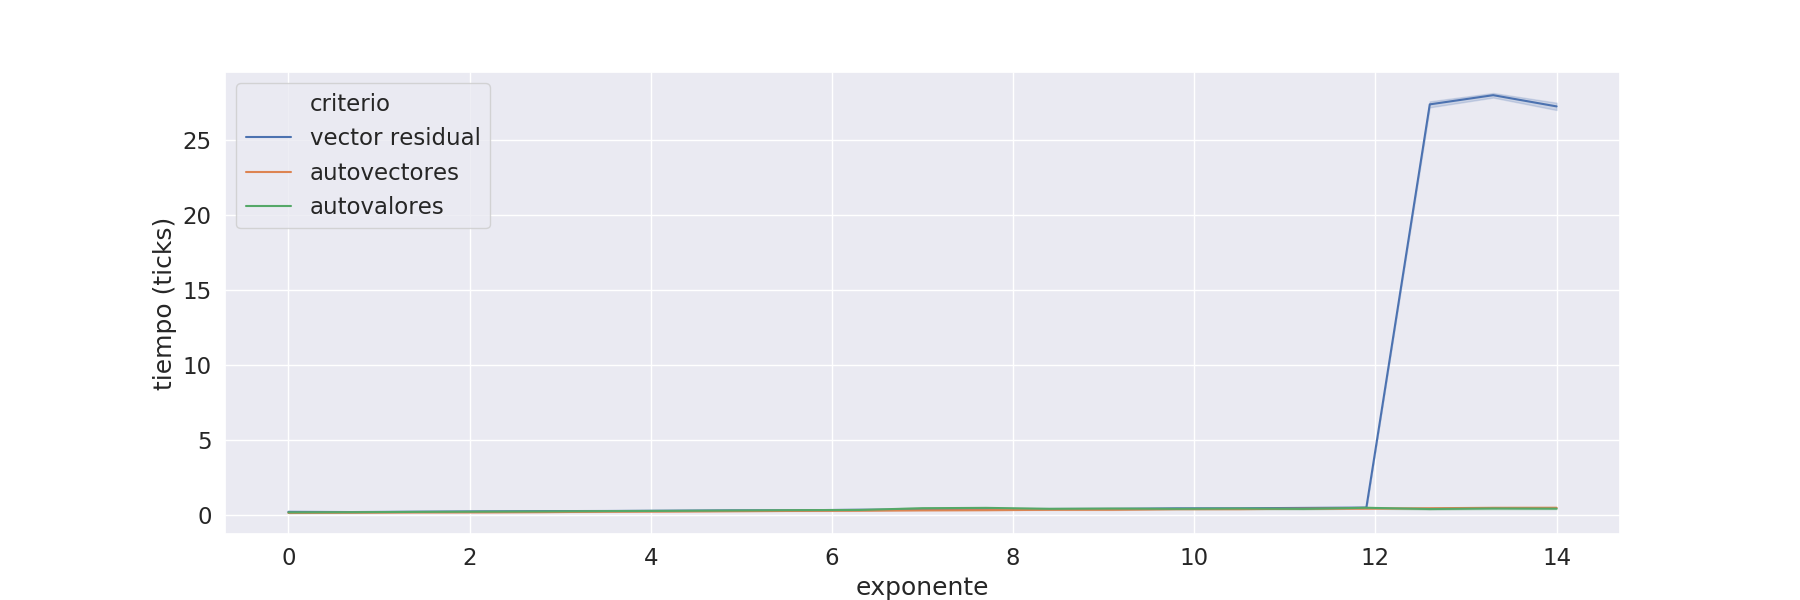
\includegraphics[width=\textwidth]{./img/tiempo_2k.png}
\centering
\caption{Progresión del tiempo medido en ticks del metodo de la potencia en función del exponente del epsilon para 2000 vectores aleatorios.}
\end{figure}

Como se puede ver en la figura () la latencia del criterio vector residual explota desmedidamente a partir del exponente $12$, como el tiempo era demasiado decidimos recortar el rango y mover el exponente solo hasta $12$ antes de pasar a medir con el dataset completo.

\begin{figure}[h]
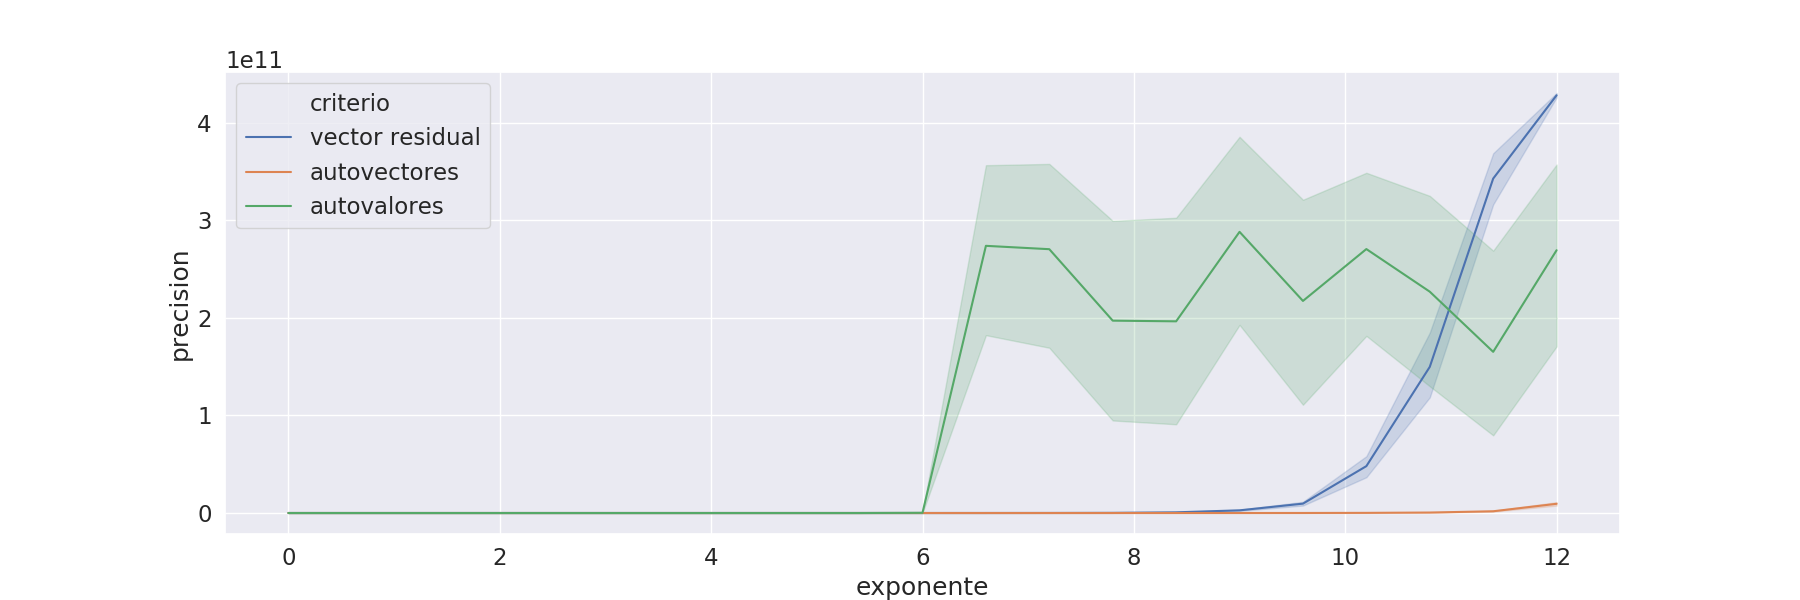
\includegraphics[width=\textwidth]{./img/precision_grande_full.png}
\centering
\caption{Progresión del tiempo medido en ticks del metodo de la potencia en función del exponente del epsilon para los 6225 vectores del dataset.}
\end{figure}

\begin{figure}[h]
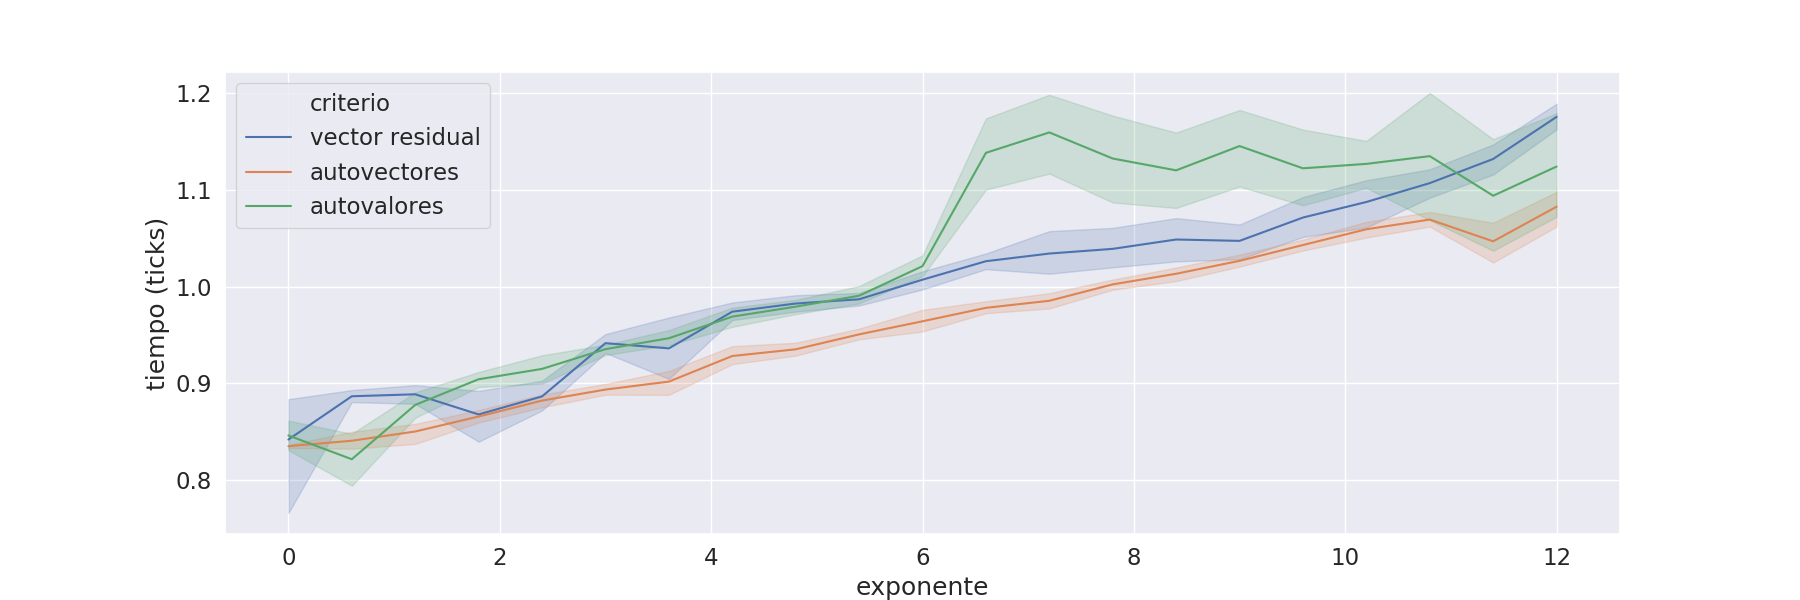
\includegraphics[width=\textwidth]{./img/tiempo_grande_full.png}
\centering
\caption{Progresión del tiempo medido en ticks del metodo de la potencia en función del exponente del epsilon para 6225 vectores del dataset.}
\end{figure}

Vemos en la figuras () que el criterio de autovalores alcanza precisiones dominantes con menos exponentes que el resto pero se mantiene inestable en variaciones y con media constante antes de que el criterio de vector residual empiece a subir de manera mucho más consistente. El criterio de autovalores recien sobre los últimos exponentes empieza a mostrar una mínima mejora.

El problema de la explosión rápida en precisión del criterio de autovalores es que viene acompañado de una explosión en latencia como indica la figura () y en el caso del criterio de vector residual para el momento en que alcanza una precisión similar al criterio de autovalores la latencia ya es considerable (tener en cuenta que la linealidad en función del exponente significa exponencialidad respecto de epsilon para la latencia). Decidimos entonces, antes de analizar los exponentes mayores a $6$ tras la explosión del criterio de autovalores y en la subida del criterio de autovectores, analizar qué sucede antes del $6$.

\begin{figure}[h]
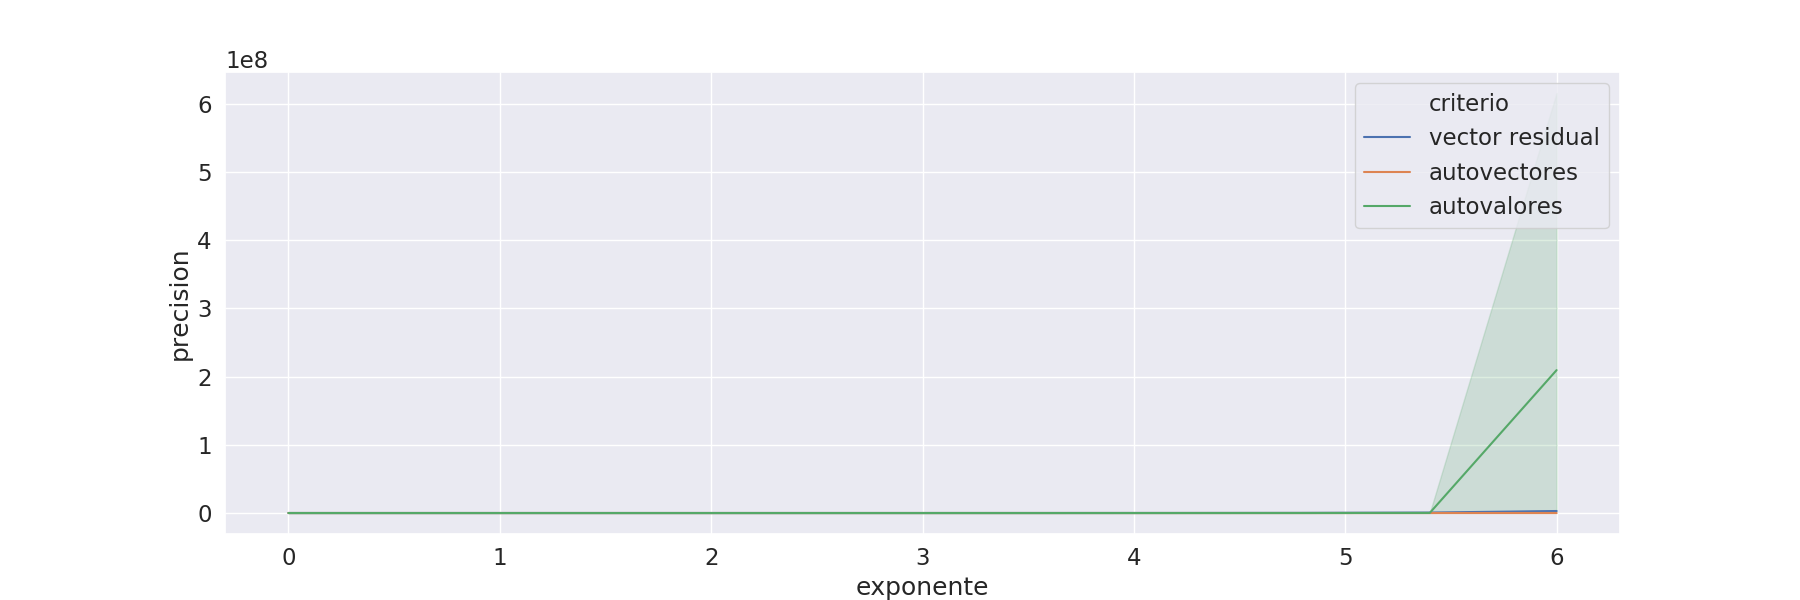
\includegraphics[width=\textwidth]{./img/precision_corto_full.png}
\centering
\caption{Progresión del tiempo medido en ticks del metodo de la potencia en función del exponente del epsilon para los 6225 vectores del dataset.}
\end{figure}

\begin{figure}[h]
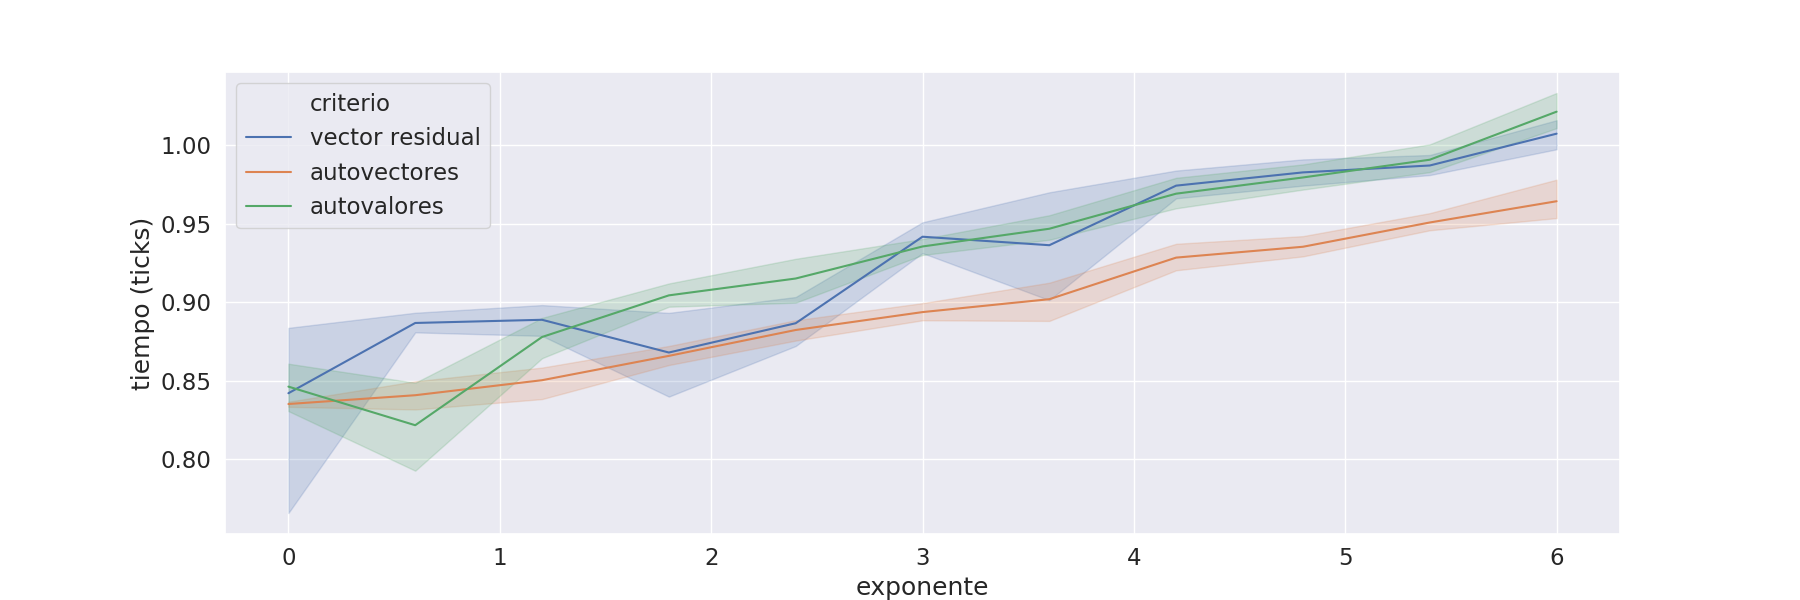
\includegraphics[width=\textwidth]{./img/tiempo_corto_full.png}
\centering
\caption{Progresión del tiempo medido en ticks del metodo de la potencia en función del exponente del epsilon para 6225 vectores del dataset.}
\end{figure}

Viendo las figuras () y () consideramos que el exponente $6$ era una interesante alternativa dado que tiene en autovalores latencia mucho menor a los exponentes mayores y aun así mostraba una mejora importante de precisión respecto de exponentes menores. Decidimos entonces, antes de pasar a comparar los valores mayores a $6$ la posibilidad de comparar el criterio de autovalores para exponente $6$ contra estos (particularmente $7$, primer valor tras la explosión) en una instancia de PCA con $k$ y $\alpha$ fijos arbitrarios, dado que solamente nos interesa medir qué tan bien funcionan en un caso práctico de PCA (que es la finalidad del método) y ninguno de los dos parámetros favorece a ninguno de los dos exponentes (sí afecta $\alpha$ en cómo se arrastra errores de precisión en el método por cuestiones de deflación, pero penaliza justamente al menos preciso de modo que no nos afecta). Al iterar corridas con tales parámetros y notar que la medida de accuracy era exactamente la misma en ambos casos con tiempos favorables (cerca de la mitad en algunos casos) para el menor exponente decidimos entonces fijar $\epsilon=10^-6$.


\subsection{Impacto del tamaño del set de entrenamiento}%
\label{sub:exp_training_set}
% 
%\subsection{Impacto del tamaño del set de entrenamiento}%
%\label{sub:exp_training_set}

% TL;DR; Como se diseño el experimento
%
Fueron tomadas mediciones sobre el comportamiento del \textit{accuracy} al
reducir el tamaño del set de entrenamiento para \knn{} con PCA.\@ Para ello se
redujo el tamaño muestral, tomando distintas sub-muestras al azar, respetando
una proporción pareja entre reseñas con calificación positiva y negativa.
% k y alpha
Se mantuvieron constantes $k$ y $\alpha$. El experimento se repitió para
distintas configuraciones de los mismos.

% acc vs N; k fijo; distintos alpha
\begin{figure}[ht]
    \centering
    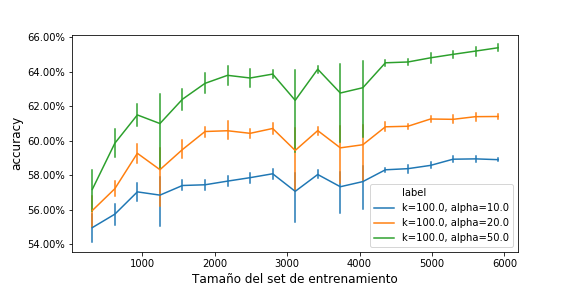
\includegraphics[width=0.6\textwidth]{img/exp_subsampling_k_fijo}
    \caption{\textit{Accuracy} obtenido al reducir el conjunto de
    entrenamiento.  Para valor fijo de $k=100$.}%
    \label{fig:subsampling_k_fijo}
\end{figure}

% acc vs N; alpha fijo; distintos k
\begin{figure}[ht]
    \centering
    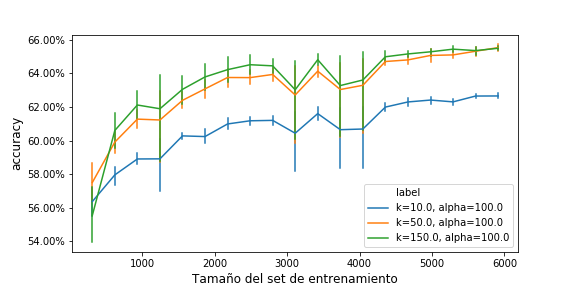
\includegraphics[width=0.6\textwidth]{img/exp_subsampling_alpha_fijo}
    \caption{\textit{Accuracy} obtenido al reducir el conjunto de
    entrenamiento.  Para valor fijo de $\alpha=100$.}%
    \label{fig:subsampling_alpha_fijo}
\end{figure}

% TL;DR; mas data => mas accuracy.
%
Puede observarse en las figuras~\ref{fig:subsampling_k_fijo}
y~\ref{fig:subsampling_alpha_fijo} que el \textit{accuracy} incrementa al
incrementar el tamaño muestral.  Por otro lado, la calidad del modelo crece
cada vez en menor medida, por lo que se cree que existe un punto a partir del
cual carece de sentido práctico incrementar el set de entrenamiento. Como el
rendimiento del modelo sigue siendo bajo, creemos que la máxima cantidad de
instancias de entrenamiento disponible, $N = 6225$, esta por debajo del tamaño
óptimo.

% TL;DR; El tamaño óptimo parece ser independiente de k y alpha.
%
Se observó el mismo comportamiento de la curva para todas las configuraciones
de $k$ y $\alpha$, por lo que se cree, el tamaño muestral óptimo es
independiente de los hiperparámetros a escoger.

% TL;DR; Se observa mayor varianza para N bajo.
%
A su vez se observa que la varianza en el \textit{accuracy} es mayor para
tamaños muestrales chicos. Esto es porque las reseñas conocidas por el modelo
pueden ser, con mayor probabilidad, poco representativas la totalidad de las
reseñas.


\subsection{Optimización de $k$ para \knn{} sin PCA}%
\label{sub:knn_sin_pca}

Para buscar una $k$ cantidad de vecinos que optimice \knn{} usamos nuevamente el dataset de \textit{imdb\_small}, iteramos un $k$ de 1 a 3000 con saltos de a 20.

Originalmente pensábamos arrancar en un rango mas adelantado dado que para $k$ pequeños sobre muestras grandes se puede correr riesgos de overfitting por puntos ``ruidosos" que estén demasiado pegados ganandole en la votación a la verdadera clase, pero como $k$ pequeños no son caros de computar los consideramos en la experimentación de todos modos.

Elegir $k$ grande tiene el problema de que los elementos de la clase de un punto quizás están todos en su vecindad inmediata y a medida que vamos buscando vecinos en zonas más alejadas vamos tendiendo a clasificar peor el punto: una clase muy densa pero rodeada de otra mas dispersa y sobrerrepresentada será peor catalogada cuanto más grande sea $k$. Si además $k$ es lo suficientemente grande (aproximadamente superando la mitad de la población total) la proporción de vecinos más cercanos se parece cada vez más y más a la proporción muestral de cada clase sobre el total, lo cual no aporta nada de información. Por lo tanto decidimos iterar solamente hasta la mitad.

Tendría sentido con este análisis que acabamos de hacer encontrar los mejores resultados en un punto intermedio en la magnitud de $k$.

\begin{figure}[h]
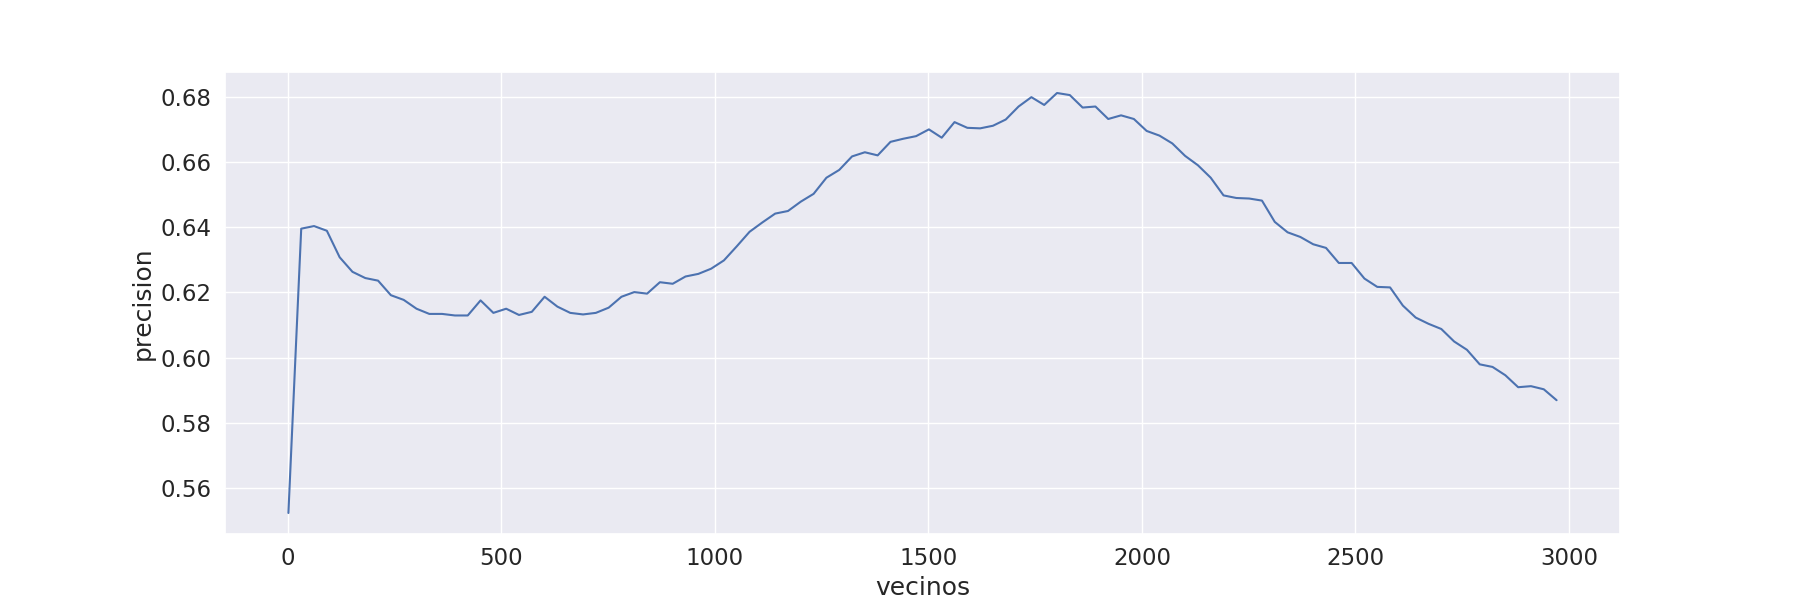
\includegraphics[width=\textwidth]{./img/knn.png}
\centering
\caption{Progresión de accuracy score de KNN en función de la cantidad de vecinos.\label{fig:knn_acc}}

\end{figure}

Como podemos apreciar en la figura \ref{fig:knn_acc}, se cumple nuestra predicción de que el accuracy score empeora conforme la cantidad de vecinos se vuelve muy grande o muy pequeña. Alcanzamos el máximo accuracy score en 0.681116 para $k=1801$ que se sitúa muy cerca de la mitad del intervalo que elegimos. Nos resulta complicado comprender por qué desciende el accuracy score en los primeros valores, especulamos con que los problemas de ruido y sesgo requieran valores de $k$ bajos pero mayores a los mínimos para que empiecen a aparecer. Otro motivo sea que si el espacio de los vectores no esté separado de manera clara existan zonas con más ruido que en el resto y que se vayan acumulando outliers de clases difusas hasta que se sale de los mismos.

\subsection{Optimización de $k$ y $\alpha$ para \knn{} con PCA}%
\label{sub:alpha_k_knn_pca}
En esta sección se buscan los hiperaparámetros de KNN y PCA que mejor
\emph{accuracy} nos brinden, sin perder de vista, pero dejando en segundo
plano, el tiempo de cómputo asociado. Además respetaremos los
parámetros de tolerancia y vocabulario encontrados en las secciones
anteriores.

\subsubsection{Performance}

El primer problema con el que nos encontramos es la amplia variación
que pueden tomar los parámetros; así como los tiempos largos que
incurre el cómputo de este método.

En particular la obtención de valores singulares para lograr el
análisis de componententes principales, que ya fué mencionada en el
apartado de \emph{power method}.

Pero también la comparación de cada nuevo punto en el predict, es
altamente dependiente de la cantidad de puntos que tiene el dataset de
entrenamientos. Como se mostró en la sección de \emph{tamaño de
  muestra}, el accuracy es sensible a la cantidad de datos de
entreamiento. Por esto es que buscamos una manera de reducir la
cantidad de comparaciones que se efectúan, sin reducir la cantidad de
datos.

Para esto usamos una estructura ``arboles kd'' o ``kd-trees'' que
permiten particionar el espacio de forma binaria por dimensión y de
esta manera permiten implementaciones mucho más eficientes de KNN.

\subsubsection{Busqueda de Parámetros}

A pesar de las optimizaciones hechas, la búsqueda es intensa en tiempo
y extensa en los valores que pueden tomar los parámetros.

Valores grandes de PCA se descartan, pues uno de las características
del método es reducir la cantidad de dimensiones de los puntos
muestrales. Es decir, en nuestro caso, elegir aquellas palabras que
tienen un mayor peso en la predicción de la clasificación.

Por otro lado valores muy pequeños pueden generar pérdida de información.

Algo similar sucede con el parámetro de los vecinos, valores muy
pequeños hacen demasiado sensible al punto a ser predecido, de su
vecindad inmediata, volviendo el método sensible a las
particularidades de los datos y por lo tanto poco fiable.

Valores muy grandes de vecindad, son computacionalmente costosos y
además se pierde el sentido de vecindad que es necesario para una
clasificación exitosa. En el caso extremo, tomar como vecinos toda la
población de entrenamiento, le asignaría a cada nuevo punto el mismo
valor: aquel mayoritario en el universo.

Los valores buscados entonces, están en algún punto intermedio. Sin
embargo, este sigue siedo un intervalo bastante grande.

Con un vocabulario del orden de las 5 mil palábras y una cantidad de
datos de entrenamiento del orden de los 15 mil, tenemos un espacio
enorme para la búsqueda.

Nuestra aproximación al problema, fue el de hacer una grilla, donde se
generan particiones del plano vecinos-componentes de forma
regular. Luego usar heurísticas de búsqueda en cada una de las celdas
de la misma. En particular se usó \emph{hill
  climbing}\cite{aiama}\footnote{o búsqueda local, intenta en cada paso
  mejorar la solución obtenida, considerando una frontera de vecinos.}
Definiendo un tamaño de grilla y un punto inicial en la misma, la
heurística se mueve a pequeños intervalos -discretos- en las cercanías
de la solución obtenida, hasta llegar a un máximo local que no puede
ser mejorado. La definición de estos pequeños intervalos, está
relacionada con el tamaño de cada celda por un lado y por otro de la
cantidad de iteraciones que hará la búsqueda local hasta alcanzar un
máximo. Esto último se debe a que los intervalos son discretos,
entonces cuanto más grandes son menos soluciones estamos considerando
y es más corto el camino hacía un máximo que no se pueda mejorar (lo
que no significa que esa un máximo real).

Esta metodología nos permite reducir mucho el espacio de búsqueda. Por
poner un ejemplo de una grilla de 100x100, donde se efectúa una
búsqueda local considerando 200 elementos, pagamos un costo
$\frac{200}{100^2} = 0,002$ menor al de explorar toda la grilla y es
sensiblemente mejor que simplemente tomar un punto arbitrario de la
misma.

Para la definición de los parámetros de la búsqueda local, tuvimos en
cuenta las consideraciones anteriores y generamos dos
grillas. Una \ref{fig:param-small} de tamaño pequeño, donde las
componentes principales se mueven entre 10 y 90 mientras que los
vecinos entre 100 y 1000 y otra \ref{fig:param-big} con una grilla de
un orden de maginitud más grande que sigue de donde dejó la anterior
en los componentes principales, pero los incrementa a un ritmo mayor,
pero mantiene las divisiones de los vecinos.

En ambos experimentos, la definición del tamaño de los pasos que hace
la búsqueda local, tuvimos en cuenta la diferente relación de aspecto
de las grillas. En el primer caso usamos un paso de 20 para los
vecinos y de 2 para las componentes principales, que guarda la
relación entre el tamaño de las aristas de cada celda. Para el segundo
experimento usamos para ambas dimensiones un paso de 10, que guarda la
relación cuadrada de la celda.

En lafiguras \ref{fig:param-small} se ve una buena zona para elegir parámetros en toda la franja 70-90 con algunos picos con pocos vecinos (200) rodeados de algunos valles, mientras que al aumentar los vecinos (800) parecíera tener menos picos pero una mejor base.

Vemos en la figura \ref{fig:param-big} que se conecta adecuadamente,
la primera fila, con la última del gráfico anterior; sugiriendo cierta
suavidad en los superficie i.e en la relación de los parámetros con la
\emph{accuracy}. El descenso más abrupto entre 500 y 600 para PCA que el
gráfico anterior se debe al cambio de escala. El descenso de la
\emph{accuracy} se puede deber a que la franja 60-600 presenta las componentes con mayor peso y todo lo que se agregue luego es ruido.

Cabe destacar que según se acostumbra en procesamiento de
lenguaje\cite{LP} natural\footnote{In general (Gale and Church, 1990)
  suggest that the vocabulary size (the number of types) grows with at
  least the square root of the number of tokens (i.e.
  $V > O(\sqrt{N})$.} la cantidad de vocabulario se suele tomar como
función creciente de la raiz cuadrada de los tokens\footnote{Tomamos
  vocabulario, como types. Los tokens son todas las entidades
  identificables en un corpus (una colección de textos) Puede incluir
  hasta signos de puntación. Los types/tipos, son las palabras
  utiles.}, y que según nuestros datos, la raiz es un valor que ronda
los 300\footnote{El valor no es exacto porque depende de como se
  consideren los tokens}; bien dentro de la franja de componentes
principales, que mencionamos antes.

\begin{figure}[h]
  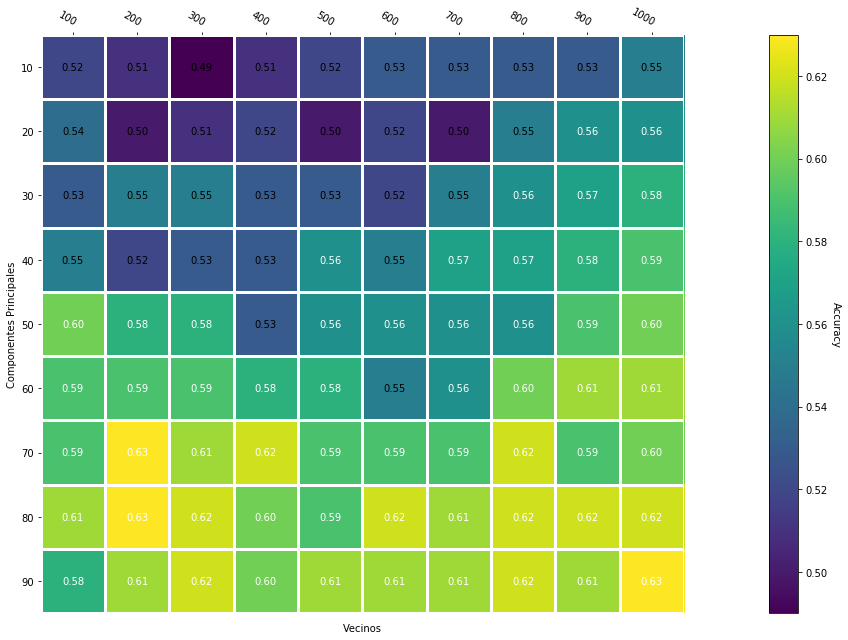
\includegraphics[width=\textwidth]{./img/parameters-search-small.png}
  \centering
  \caption{Resultado de la busqueda local sobre cada región
    \textbf{pequeña} de k100x$\alpha$10. Usando la implementación de
    sklearn. En cada una de las celdas, se corrió una búsqueda local,
    comenzando en el valor mostrado en los ejes hasta alcanzar un
    máximo local. El promedio de corridas es aproximadamente de 8,
    versus una cantidad de puntos de \textbf{1000}. Se muestran sobre
    el color, el accuracy logrado por el máximo local.}
  \label{fig:param-small}
\end{figure}

\begin{figure}[h]
  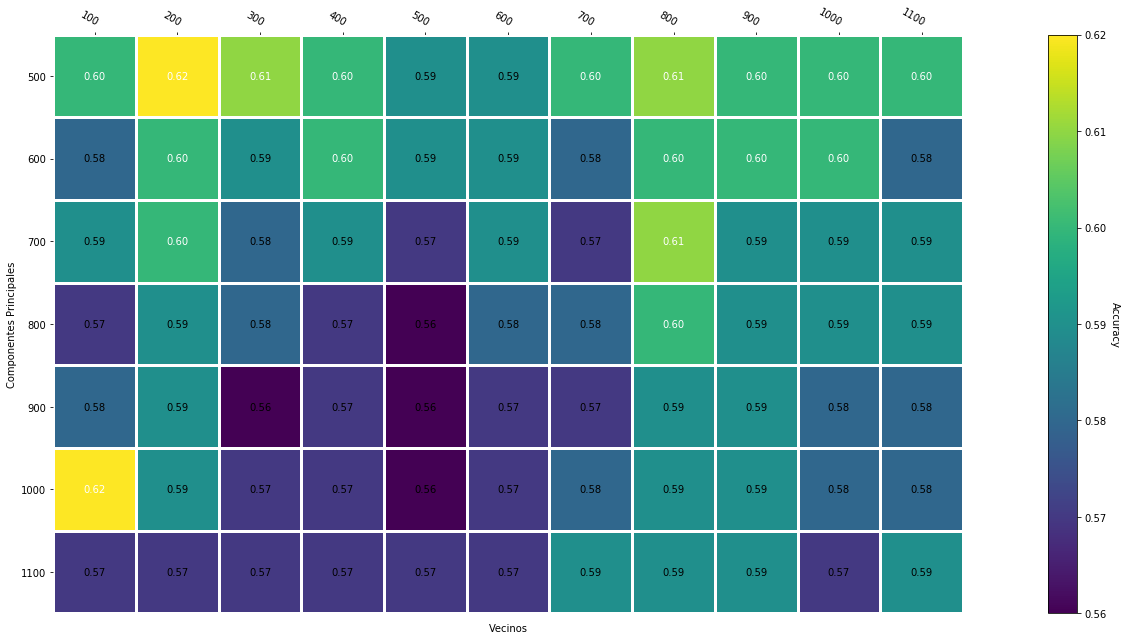
\includegraphics[width=\textwidth]{./img/parameters-search-big.png}
  \centering
  \caption{Resultado de la busqueda local sobre cada región
    \textbf{grande} de k100x$\alpha$100. Usando la
    implementación de sklearn. En cada una de las celdas, se corrió
    una búsqueda local, comenzando en el valor mostrado en los ejes
    hasta alcanzar un \textbf{máximo local}. El promedio de corridas
    es aproximadamente de 12, versus una cantidad de puntos de
    \textbf{10000}. Se muestran sobre el color, el accuracy logrado
    por el máximo local.}
    \label{fig:param-big}
\end{figure}


